\section{Exercise 1}

Consider the one-dimensional Laplace equation
\begin{equation*}
u_{xx} = f(x) \qquad (0 < x < 1)
\end{equation*}
with the source term $f(x) = x + \cos(2 \pi x)$, subject to different kinds of boundary conditions
\begin{equation*}
\begin{aligned}
u(0) &= a, &\quad u(1) &= b &\qquad& \text{(Dirichlet-Dirichlet)} \\
u_x(0) &= a, &\quad u_x(1) &= b &\qquad& \text{(Neumann-Neumann)} \\
u(0) &= a, &\quad u_x(1) &= b &\qquad& \text{(Dirichlet-Neumann)}. \\
\end{aligned}
\end{equation*}

An analytical solution is
\begin{equation*}
u(x) = C_1 + C_2 x + \frac{1}{6}x^3 - \frac{1}{4 \pi^2}\cos(2 \pi x)),
\end{equation*}
where the constants $C_1$ and $C_2$ are determined from two boundary conditions.
Note that when Neumann-Neumann boundary conditions are imposed, $C_1$ is undetermined and so the solution is determined only up to a constant.

Grid:
\begin{center}
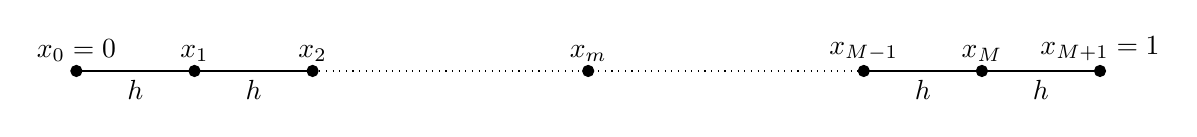
\begin{tikzpicture}
\draw (0,0) -- (3,0);
\draw[dotted] (3,0) -- (10,0);
\draw (10,0) -- (13,0);
\filldraw (0.0,0) circle (2pt) node[anchor=south] {$x_0 = 0$};
\filldraw (1.5,0) circle (2pt) node[anchor=south] {$x_1$};
\filldraw (3.0,0) circle (2pt) node[anchor=south] {$x_2$};
\filldraw (6.5,0) circle (2pt) node[anchor=south] {$x_m$};
\filldraw (10.0,0) circle (2pt) node[anchor=south] {$x_{M-1}$};
\filldraw (11.5,0) circle (2pt) node[anchor=south] {$x_{M}$};
\filldraw (13.0,0) circle (2pt) node[anchor=south] {$x_{M+1} = 1$};
\node[anchor=north] at (0.75, 0) {$h$};
\node[anchor=north] at (2.25, 0) {$h$};
\node[anchor=north] at (10.75, 0) {$h$};
\node[anchor=north] at (12.25, 0) {$h$};
\end{tikzpicture}
\end{center}

Inner points:
\begin{equation*}
\frac{U_{m+1} - 2 U_m + U_{m-1}}{h^2} = f(x_m)
\end{equation*}
Dirichlet, left:
\begin{equation*}
u(0) = U_0
\end{equation*}
Von-Neumann, left, 2nd order:
\begin{equation*}
u_x(0) \approx -\frac{(3/2)U_0 -2U_1 + (1/2)U_2}{h}
\end{equation*}

Discretized equation:
\begin{equation*}
\renewcommand{\arraystretch}{2.8} % stretch matrix vertically to make it square
\begin{bmatrix}
-2/h^2 & +1/h^2  & 0 & \cdots & 0 \\
+1/h^2  & -2/h^2 & +1/h^2  & \ddots & \vdots \\
0 & \ddots & \ddots & \ddots & 0 \\
\vdots & \ddots & +1/h^2 & -2/h^2 & +1/h^2\\
0 & \cdots & -1/2h & +2/h & -3/2h  \\
\end{bmatrix}
\begin{bmatrix}
U_1 \\ U_2 \\ \vdots \\ U_M \\ U_{M+1} \\
\end{bmatrix}
=
\begin{bmatrix}
f(x_1) - \alpha/h^2 \\ f(x_2) \\ \vdots \\ f(x_M) \\ \sigma \\
\end{bmatrix}
\end{equation*}

\begin{figure}
  \centering
  \begin{tikzpicture}
\begin{loglogaxis}[
  title=Error functions,
  xlabel={$M$},
  ylabel={$e_l$},
  legend pos=south west,
  ]

  \addplot table[y index=1] {exercise1/a_error.dat}
  coordinate [pos=0.24] (A)
  coordinate [pos=0.8] (B);
  \addplot table[y index=2] {exercise1/a_error.dat};
  \addplot table[y index=3] {exercise1/a_error.dat};

  \draw (A) -| (B)
  node [pos=0.25, anchor=south] {1}  %% Random value
  node [pos=0.75, anchor=west] {-1};

  \legend{$L_2$ discrete, $L_2$ continous step, $L_2$ continous interpolatino};
\end{loglogaxis}
\end{tikzpicture}

  \caption{Nice fig}
\end{figure}
